\hyt{triandele}
\song{Tři andělé} \interpret{plihal}{Karel Plíhal}

\vers{1}{

\vspace{-53pt}
\hspace{20pt}
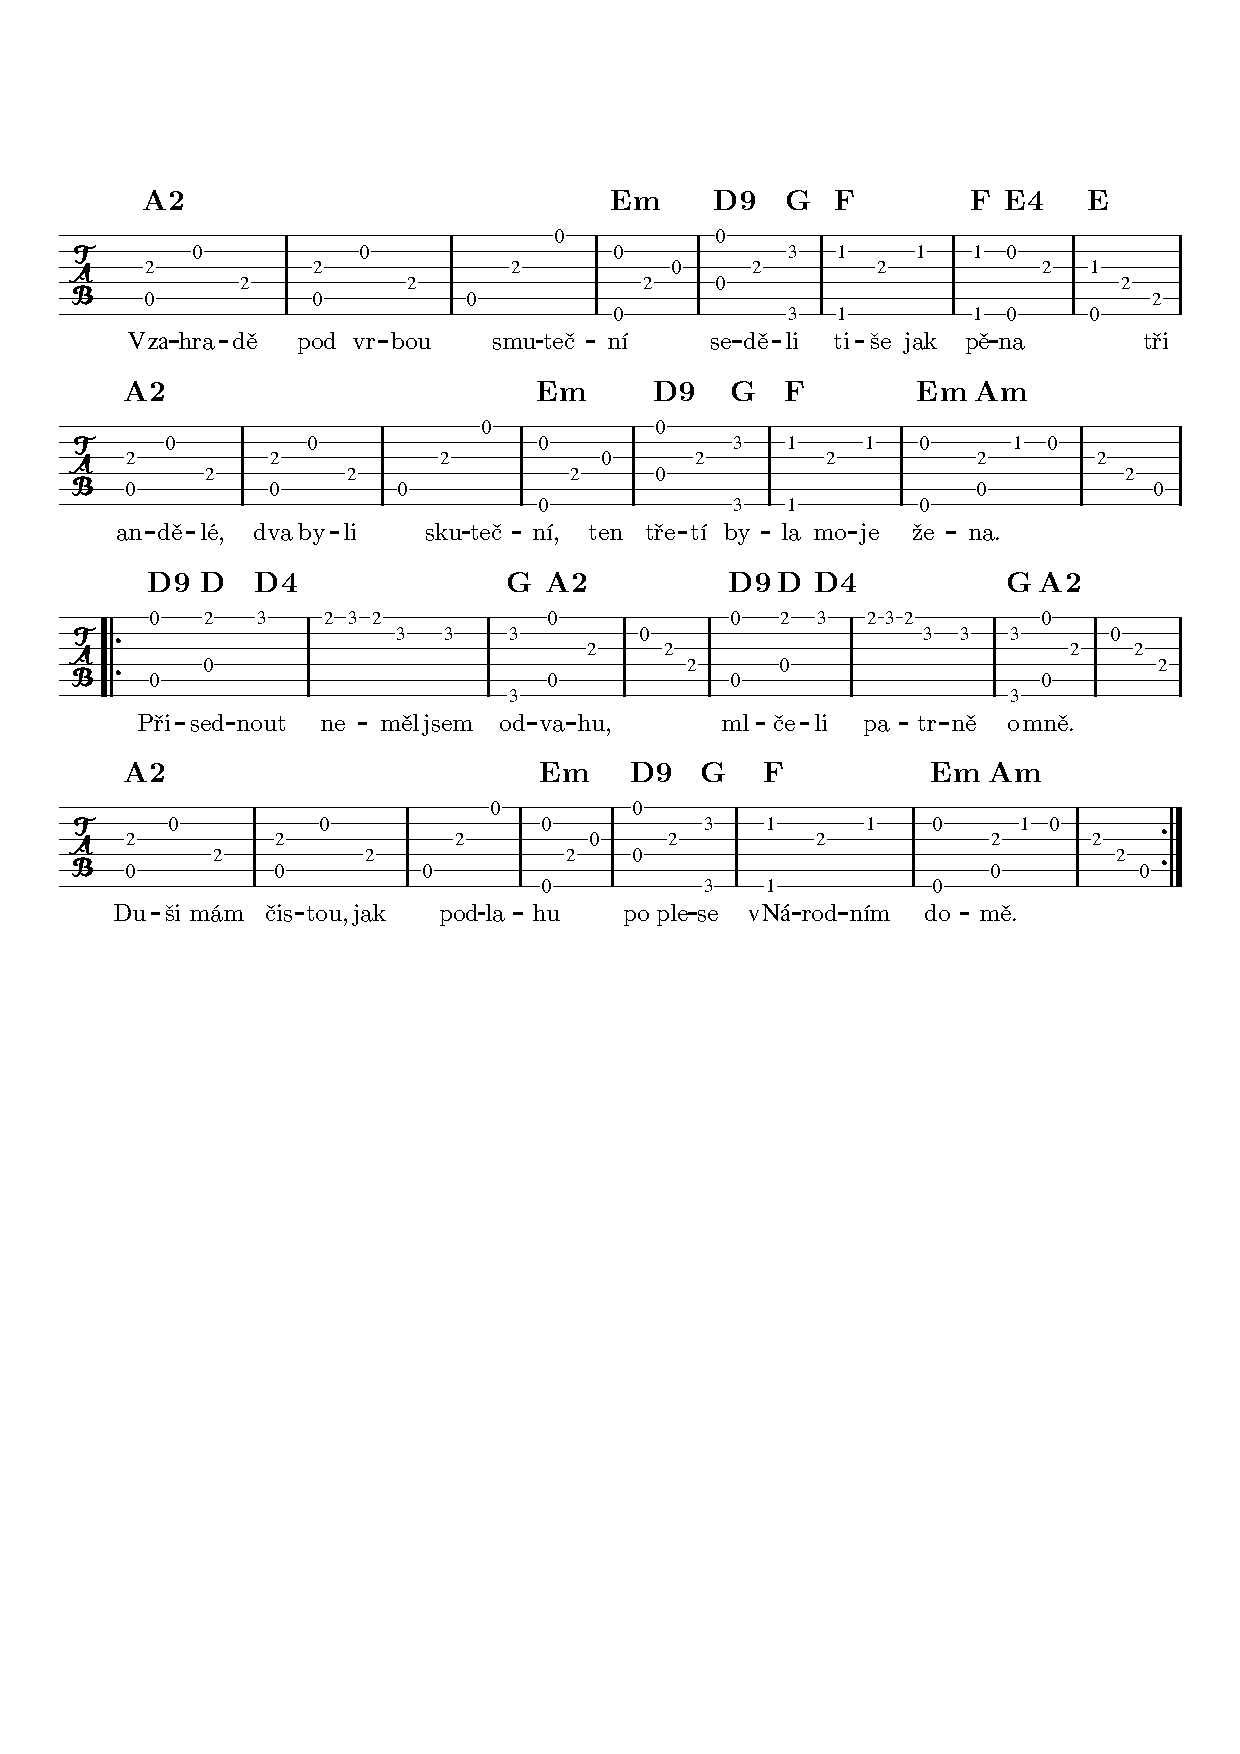
\includegraphics[width=\linewidth]{scores/triandele.pdf}
}

\vers{2}{
Určitě skončili u cifer, sčítajíc všechny mé hříchy,\\
až si to přebere Lucifer, nejspíš se potrhá smíchy.\\
\rep{Obloha zčernala sazemi z komínů vesmírných lodí,\\
dokud jsou andělé na Zemi, nic zlého se nepřihodí.}
}
\newpage
